\documentclass[12pt]{article}

\usepackage{allrunes}
\usepackage{amsmath}
\usepackage[magyar]{babel}
\usepackage[T1]{fontenc}
\usepackage[utf8]{inputenc}
\usepackage{fixltx2e}
\usepackage{multirow}
\usepackage{hyperref}
\usepackage{amsfonts}
\usepackage{amsthm}
\usepackage{amssymb}

\usepackage{geometry}
\geometry{a4paper,
		     tmargin = 35mm, 
		     lmargin = 30mm,
		     rmargin = 30mm,
		     bmargin = 30mm}

\theoremstyle{plain}
\usepackage{graphicx}

%\usepackage{gensymb}
\usepackage{float}
\usepackage{indentfirst}

%linkek 
\newcommand{\ndurl}[2]{\textit{\href{#1}{\underline{#2}}}}

\renewcommand\thesection{\Roman{section}}

%% New commands
\newcommand{\ket}[1]{\left| #1 \right >}
\newcommand{\bra}[1]{\left < #1 \right |}
\newcommand{\braket}[2]{\left < #1 \middle | #2 \right>}
\newcommand{\ketbra}[2]{\left | #1 \right> \left< #2 \right |}
\newcommand{\norm}[1]{\left{||} #1 \right{||}}
\newcommand{\commut}[2]{\left [ #1 , #2 \right]}

\newcommand{\dd}{\textrm{d}}

\newcommand{\mev}{~\textrm{MeV}}
\newcommand{\fm}{~\textrm{fm}}

%% Pauli matrices
\newcommand{\sigx}{\sigma_x}
\newcommand{\sigy}{\sigma_y}
\newcommand{\sigz}{\sigma_z}

\newcommand{\paulix}{
    \left( \begin{array}{cc}
        0 & 1 \\
        1 & 0
    \end{array}
    \right)
}
\newcommand{\pauliy}{
    \left( \begin{array}{cc}
        0 & -i \\
        i & 0
    \end{array}
    \right)
}
\newcommand{\pauliz}{
    \left( \begin{array}{cc}
        1 & 0 \\
        0 & -1
    \end{array}
    \right)
}
\newtheorem*{theorem*}{Tétel}
\newtheorem*{def*}{Definíció}
\newtheorem*{pld*}{Példa}
\newtheorem*{megj}{Megjegyzés}

\linespread{1.2}

\begin{document}
\title{Röntgen vonalprofil analízis}
\author{Olar Alex}
\date{2018}

\maketitle
\vspace*{2.5cm}
\begin{figure}[h!]
	\begin{center}
		
\includegraphics[width=0.7\textwidth]{../elte.jpg}
	\end{center}
\end{figure}

\newpage

\tableofcontents

\newpage


\section{Bevezetés}

\par A mérés egy olyan anyagszerkezeti vázsgálatra alkalmas módszer, amivel a minta szemcseméretét, diszlokációsűrűségét tudtuk meghatározni. Ennek
során forgóanódos röntgen diffraktométert használtunk, a diffraktogram mentésére pedig imaging plate-et. Az adatokat Originnel értékeltül ki,
a vonalkiszélesedést a Williamson-Hall módszerrel vizsgáltuk, részletesen pedig a CMWP módszerrel nyertünk ki adatokat. A jegyzet \cite{rvaleiras}
ezeket részletesen tárgyalja.

\subsection{Mérésleírás}

\vspace{.2cm}

\par Nagy intenzitású röntgen nyalábot bocsátottunk a mintára, a nyaláb $\lambda(\textrm{CuK}_{\alpha_1}) = 1.15406\AA$ hullámhosszúságú
monokromátor segítségével szűrtük meg. A mintától $d=220 mm$ távolságra elhelyezett imaging plate lemezek segítségével rögzítettük 
a Debye-Scherrer gyűrűket. Az intenzitást a $2\theta$ függvényében ábrázoltuk a laboron használt program segítségével,
így egy spektrumot kaptunk.

\section{Williamson-Hall módszer}

\vspace{.2cm}

\par A Williamson-Hall módszerrel megállapíthatjuk a vonalkiszélesedés okát. A csúcsokra Lorentz-görbét illesztettünk
a szofver segítségével, majd az illesztésből meghatároztk a $\Delta (2\theta)$ szélesség értékeket. Ezután a félértékszélességet:

\vspace{.2cm}

\begin{equation*}
	FWHM = \frac{\Delta (2\theta) \cos(\theta)}{\lambda}
	\label{eq:fwhm}
\end{equation*}

\vspace{.2cm}

\par A diffrakciós vektor hossza pedig:

\vspace{.2cm}

\begin{equation*}
	g = \frac{2\sin\theta}{\lambda}
	\label{eq:diffvec}
\end{equation*}

\vspace{.2cm}

\par Mivel a Williamson-Hall grafikonon (\ref{fig:wh_1}. ábra) nem monoton növekedést látunk, ebből következik, hogy kevert típusú
diszlokációk okozzák a vonalkiszélesedést. Ezért a félértékszélességet $g$ helyett $g^2C$ függvényében kell ábrázolni, ahol

\vspace{.2cm}

\begin{equation*}
	C = C_{h00}(1-qH^2)
\end{equation*}

\vspace{.2cm}

\par az ún. átlagos diszlokáció kontraszt faktor. $C_{h00}$ a $h00$ síkra vonatkozó átlagos diszlokáció kontraszt faktor,

\vspace{.2cm}

\begin{equation*}
	H^2 = \frac{h^2k^2 + h^2l^2 + k^2l^2}{(h^2+k^2+l^2)^2}
\end{equation*}

\vspace{.2cm}

\par $q$ pedig az anyag rugalmas tulajdonságaiból és a diszlokációk típsától függő paraméter, amit az illesztés alapján kapunk meg.

\vspace{.2cm}

\begin{table}[H]
	\begin{center}
		\begin{tabular}{|c|c|c|c|c|c|c|} \hline
			$2\theta$ & $hkl$ & $\Delta 2\theta$ & $FWHM$  & $g$      & $H^2$     & $g^2 C$   \\ \hline
			$43.527$  & $111$ & $0.134083$       & $0.808$ & $4.8134$ & $0.333$   & $1.93664$ \\ \hline
			$50.304$  & $200$ & $0.231322$       & $1.359$ & $5.5176$ & $0.0$     & $9.28540$ \\ \hline
			$74.175$  & $220$ & $0.261849$       & $1.355$ & $7.8285$ & $0.25$    & $8.50501$ \\ \hline
			$89.853$  & $311$ & $0.407956$       & $1.874$ & $9.1678$ & $0.15702$ & $16.8600$ \\ \hline
			$95.242$  & $222$ & $0.288552$       & $1.262$ & $9.5898$ & $0.333$   & $7.68713$ \\ \hline
			$116.853$ & $400$ & $0.771052$       & $2.620$ & $11.060$ & $0.0$     & $37.3102$ \\ \hline
		\end{tabular}
		\caption{ $2\theta$ értékek, a hozzájuk tartozó Miller-indexek és a félérték-szélességek.}
	\end{center}
	\label{table:fwhm}
\end{table}

\vspace{.2cm}

\par A mérésből számolt $2\theta$ értékeket, a félérték szélességeket, valamint a kiszámolt $g^2C$ értékeket
\aref{table:fwhm}. táblázatban foglaltam össze. A $g^2C$ függvényében ábrázolt pontok, valamint az illesztett
parabola a \ref{fig:wh_2}. ábrán láthatók.

\vspace{.2cm}

\begin{figure}[H]
	\begin{center}
		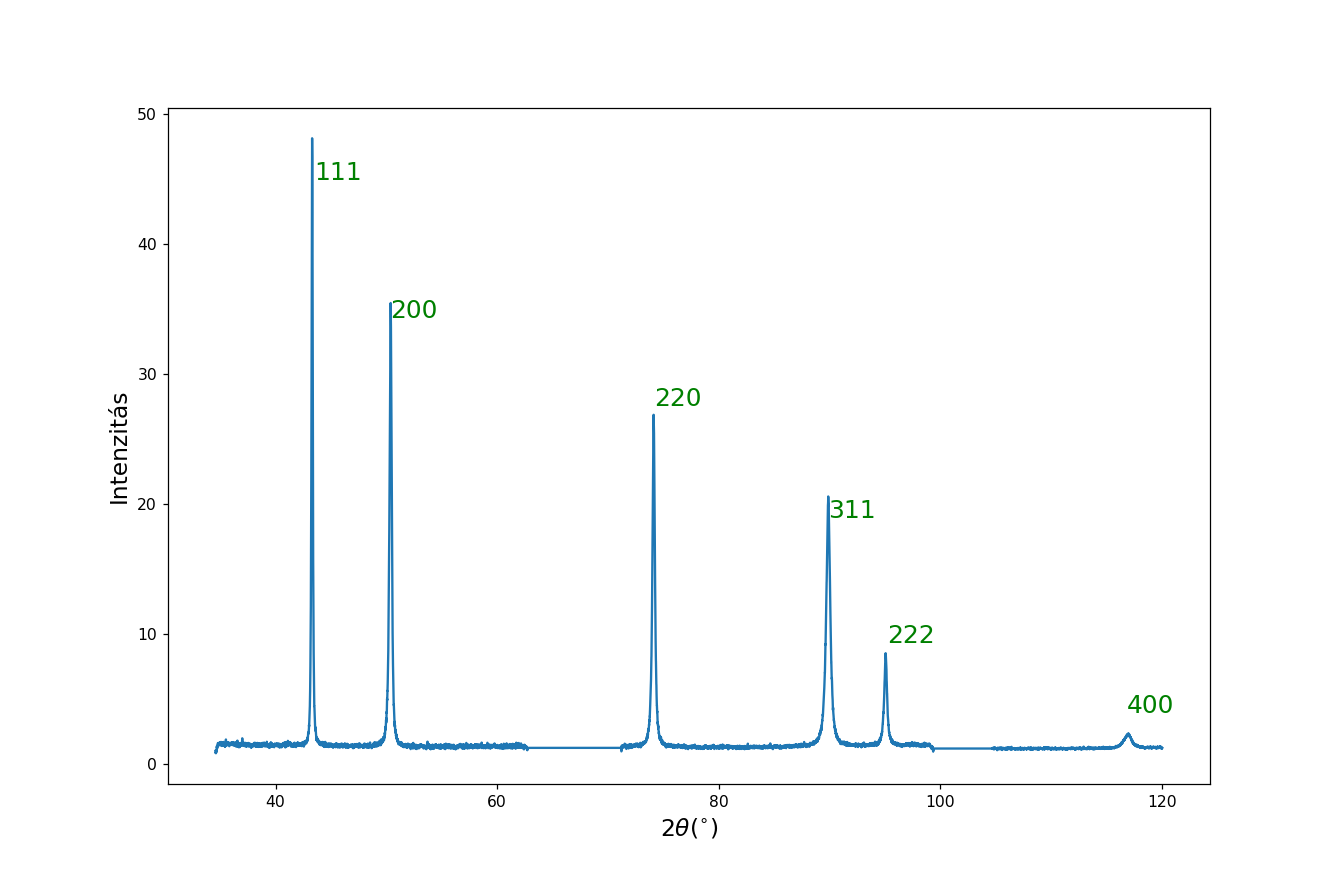
\includegraphics[width=0.85\textwidth]{./xray-lab/cuspectra.png}
		\caption{Cu minta diffrakciós spektruma és a csúcsokhoz tartozó Miller-indexek.}
	\end{center}
	\label{fig:cuspectra}
\end{figure}

\begin{figure}[H]
	\begin{center}
		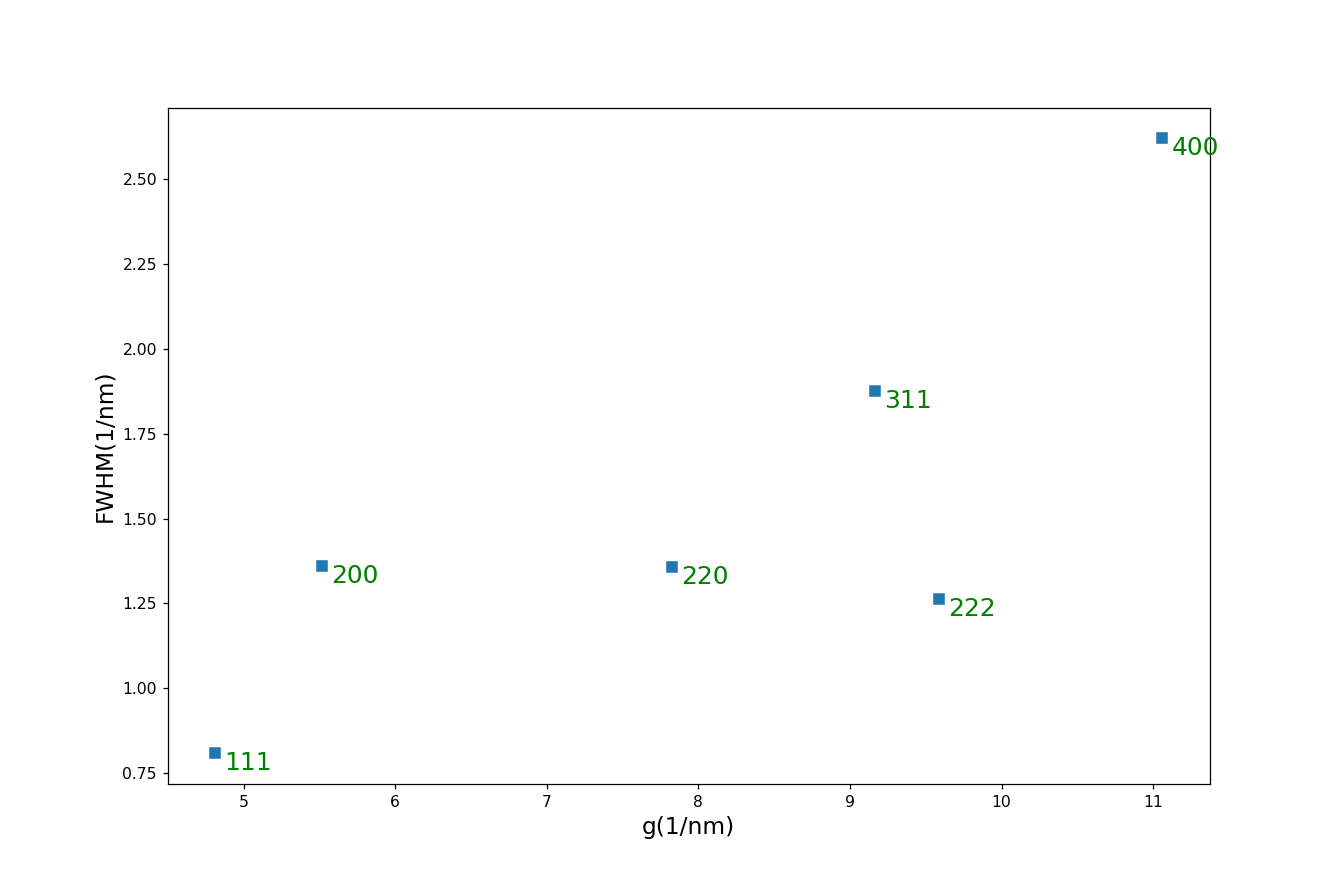
\includegraphics[width=0.85\textwidth]{./xray-lab/wh1.png}
		\caption{Williamson-Hall ábra illesztés és korrekció nélkül}
	\end{center}
	\label{fig:wh_1}
\end{figure}

\begin{figure}[H]
	\begin{center}
		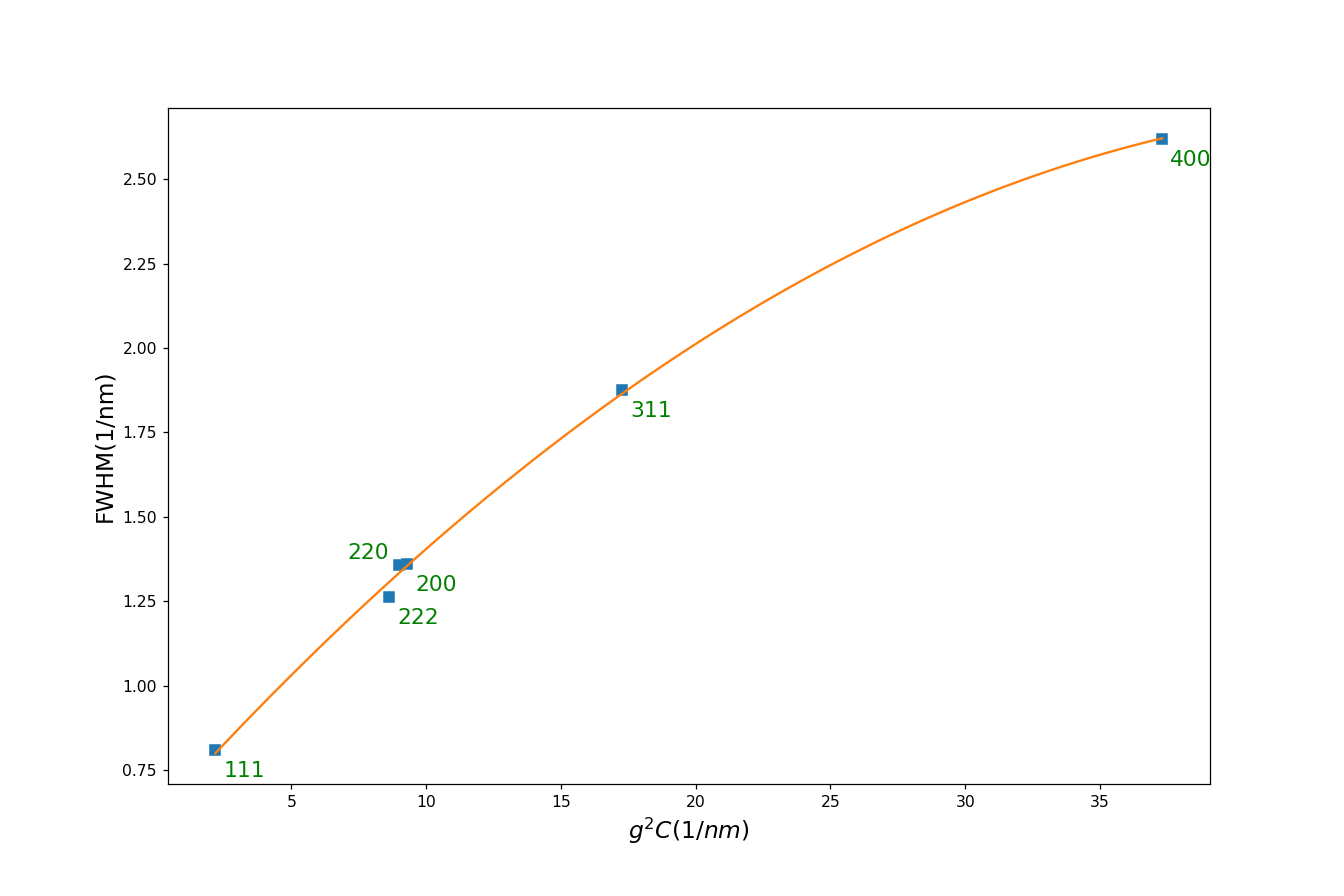
\includegraphics[width=0.85\textwidth]{./xray-lab/wh2.png}
		\caption{Williamson-Hall ábra és az illesztett parabola}
	\end{center}
	\label{fig:wh_}
\end{figure}

\vspace{.2cm}

\par Az illesztés $q=2.078$ érték esetében volt a legjobb, ekkor az illesztett $ax^2+bx+c$ egyenletű parabola paraméterei:

\vspace{.2cm}

\begin{itemize}
	\item $a=-0.0009776\pm7\cdot10^{-9}$
	\item $b=0.089647\pm1.2\cdot10^{-5}$
	\item $c=0.6370\pm6.3\cdot10^{-4}$
\end{itemize}

\section{CMWP módszer}

\vspace{.3cm}

\par A CMWP módszer elvégzésére segítségül szolgált egy szoftver, ami a diffraktogramot automatikusan kiértékelte.
Bemeneti paraméterként megadtuk a rácsparamétert ($a=0.3615nm$), a kontrasztfaktort ($C_{h00}=0.30525$),
és a hullámhosszt ($\lambda=0.15406nm$), a program elvégezte az illesztést és kiszámolta a mérérs és az illesztés közötti eltérést is:

\vspace{.2cm}

\begin{table}[H]
	\begin{center}
		\begin{tabular}{|c|c|c|} \hline
			Paraméter & Skálázatlan        & Skálázott \\ \hline
			$a$       & $2.0787 \pm 0.005$ & $2.07873$ \\ \hline
			$b$       & $0.7526 \pm 0.001$ & $3.76314$ \\ \hline
			$c$       & $1.2683 \pm 0.007$ & $0.63415$ \\ \hline
			$d$       & $1.3257 \pm 0.006$ & $66.2855$ \\ \hline
			$e$       & $3.6352 \pm 0.050$ & $0.07270$ \\ \hline
		\end{tabular}
		\caption{CMWP algoritmus illesztett paraméterei.}
	\end{center}
	\label{table:cmwp}
\end{table}

\begin{figure}[H]
	\begin{center}
		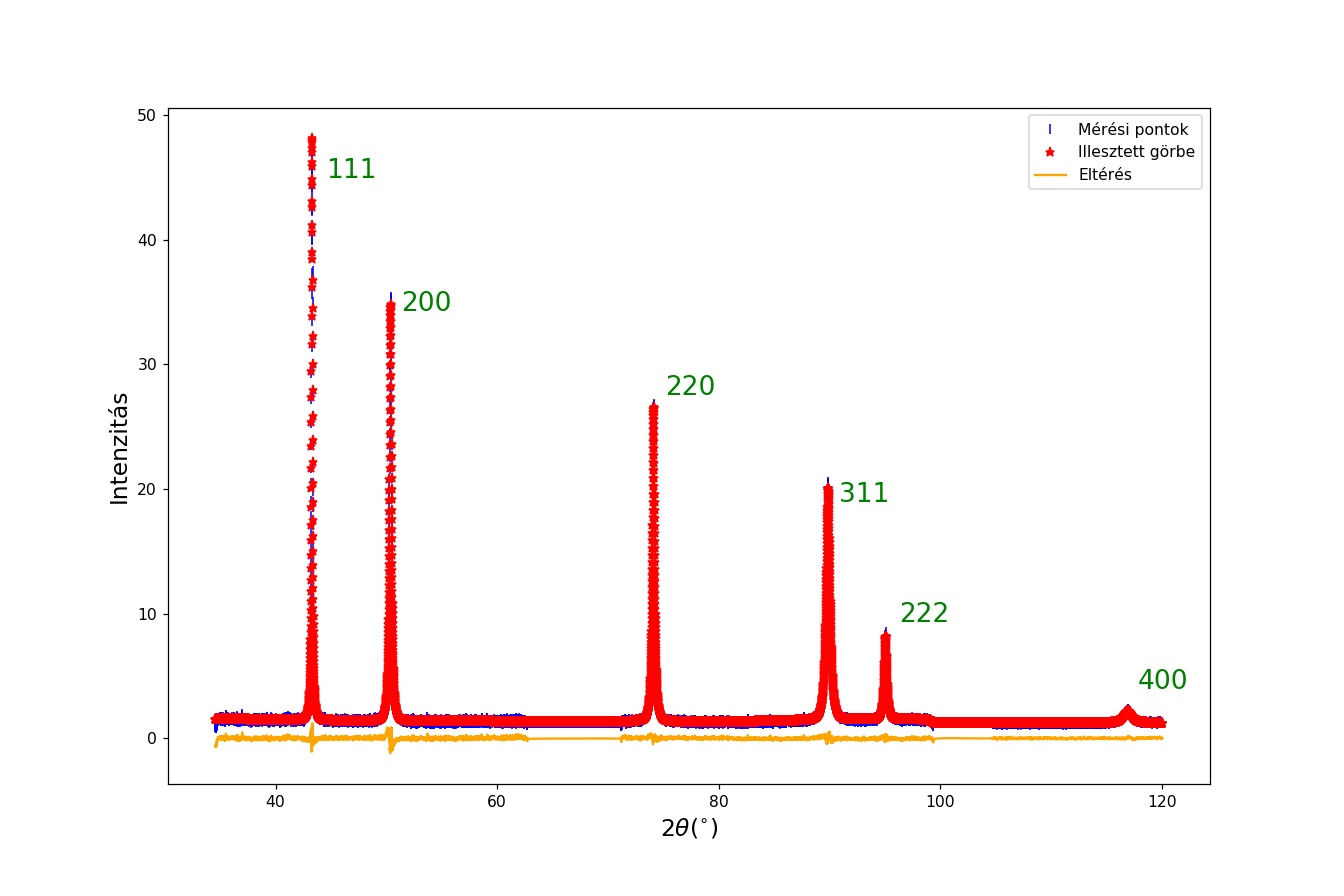
\includegraphics[width=0.85\textwidth]{./xray-lab/cmwp.png}
		\caption{Williamson-Hall ábra és az illesztett parabola}
	\end{center}
	\label{fig:cmwp}
\end{figure}

\vspace{.2cm}

\par A lognormális eloszlás paraméterei és a diszlokációkat jellemző paraméterek:

\vspace{.2cm}

\begin{itemize}
	\item $m = \exp(b) = 43.08\pm0.1~nm$ átlag
	\item $\sigma = c/\sqrt{2} = 0.44841\pm0.004$ szórás
	\item $\rho = \frac{2}{\pi (bd)^2}=0.00221779 \pm 0.00002~(1/nm)^2$ diszlokáció sűrűség
	\item $q  = a = 2.0787$ a diszlokációk típusát jellemző paraméter
	\item $R_e^*=e^{-1/4}/(2e)=5.35597\pm0.08~nm$ külső levágási sugár
	\item $M^*=(R_e^*)\cdot\sqrt{\rho}=0.252231\pm0.004$ diszlokáció elrendeződési paraméter
\end{itemize}

\vspace{.2cm}

\par Ezen paraméterek ismeretében kiszámítható a szemcsék számtani, felületi és térfogati átlaga:

\begin{eqnarray}
	\left<x_{sz}\right> = m\exp{0.5\sigma^2} = 47.636 \pm 0.25 nm\\
	\left<x_{f}\right> = m\exp{2.5\sigma^2} = 71.21 \pm 1.2nm\\
	\left<x_{tf}\right> = m\exp{3.5\sigma^2} = 87.075 \pm 2.3nm
\end{eqnarray}

\vspace{.2cm}

\section{Konklúzió}

\vspace{.2cm}

\par A mérés során megismerkedhettünk egy mai is használt anyagfizikai
mérési módszerrel. A mérési adataink kellően pontosak és a kiértékelés során
körültekintően jártunk el.

\newpage

\bibliographystyle{plain}
\bibliography{references}

\end{document}